\documentclass[a4paper]{article}

\usepackage{graphicx} % Enable including images.
\usepackage[hidelinks]{hyperref} % Link citations to their corresponding references.
\usepackage[utf8]{inputenc} % Use UTF-8 input encoding.
\usepackage[numbers]{natbib} % Enable the use of the 'citeauthor' command.
\usepackage{parskip} % Add spacing between paragraphs and don't indent the first line.

\begin{document}

\section{Feedforward} \label{section_background}
Feedforward is a relatively new concept that has been the subject of much confusion, and thus it is worth clarifying. Feedforward was first defined by \citeauthor{djajadiningrat2002but} in \citeyear{djajadiningrat2002but} as 


Feedforward is:
	communication of the purpose of an action. \cite{djajadiningrat2002but}

	informs the user about what the result of his action will be. Inviting the appropriate action is a prerequisite for feedforward but it is not sufficient. The product also needs to communicate what the user can expect. \cite{djajadiningrat2002but}

	a HCI design technique that aims at making explicit the action that is required to perform an interaction and its effect. \cite{chueke2016perceptible}
	
	intelligibility information that is provided before an event takes place. \cite{vermeulen2013intelligibility}
	
	communicating what will be the result of an action


%Feedforward hasn't always been clearly defined. People don't know it exists, confuse it with other concepts (like affordances) or use different names for it (signifiers). Let's now define what feedforward is, according to different definitions.
%
%Perceptible affordances and feedforward for gestural interfaces: Assessing effectiveness of gesture acquisition with unfamiliar interactions \cite{chueke2016perceptible}
%
%Intelligibility Required: How to Make Us Look Smart Again \cite{vermeulen2013intelligibility}
%
%Crossing the bridge over Norman's Gulf of Execution: revealing feedforward's true identity \cite{vermeulen2013crossing}
%
%When it is not possible for designers of electronic products to establish direct couplings between action and function information is needed. Information that can guide the user’s actions towards the intended function. This is the area of feedback and feedforward. \cite{wensveen2004interaction}
%
%With feedforward we mean communication of the purpose of an action. \cite{djajadiningrat2002but}
%
%For a control to say something about the function that it triggers, we need to move away from designs in which all controls look the same. \cite{djajadiningrat2004tangible} 
%
%As pointed out by Norman \cite{norman2013design}, controls of electronic products often look highly similar and require the same actions. If all controls look the same and feel the same, the only way left to make a product communicate its functions is through icons and text labels, requiring reading and interpretation. \cite{djajadiningrat2004tangible}
%
%Signifiers are the most important addition to the chapter, a concept first introduced in my book Living with Complexity. The first edition had a focus upon affordances, but although affordances make sense for interaction with physical objects, they are confusing when dealing with virtual ones. As a result, affordances have created much confusion in the world of design. Affordances define what actions are possible. Signifiers specify how people discover those possibilities: signifiers are signs, perceptible signals of what can be done. Signifiers are of far more importance to designers than are affordances. Hence, the extended treatment. \cite{norman2013design}
%
%Preview important in the real world because it is often not possible to undo an action. \cite{rekimoto2003presense}

\section{Related Work} \label{section_related_work}
Since feedforward, AR and ubicomp are all recent topics of research, literature combining the three is still scarce (but it does exist \cite{park2014previewable, vermeulen2009bet}). However, there is a moderate set of works that combine at least two of the topics, or that bring forth some relevant technique. The discussion of these works is divided up into some general categories, to more easily make connections and to limit repetition.

\subsection{Gestures} \label{subsection_gestures}
PreSense: interaction techniques for finger sensing input devices \cite{rekimoto2003presense}

OctoPocus explores the use of feedforward in on-screen gesture-based commands \cite{bau2008octopocus}. When the user initiates a command, for each possible gesture a labeled path radiates from the cursor, giving the user feedforward on what will happen if they move the cursor in a particular way. The accompanied user study indicates that this approach allows for lower overhead in time than when using traditional help menus, that it is less error-prone, allows for ``in situ'' learning, and that it is generally preferred by users.

Enhanced feed-forward for a user aware multi-touch device \cite{freitag2012enhanced}



%\subsection{AR Projectors and the Feedforward Torch} \label{subsection_ar_projectors_feedforward_torch}
%Multiple studies have touched on the use of projectors to augment environments with feedforward information. We name two more recent ones, the first of which  is conducted by \citeauthor{vermeulen2009bet} \cite{vermeulen2009bet}. In this study, a series of static and steerable projectors display icons and labels on the walls of a room, representing the present input/output devices and their available actions, along with how to trigger them. Although this study draws no conclusions regarding feedforward (since only an informal first-use study was conducted that focused on the effects of real-time feedback), the concept certainly remains relevant to us. The second study concerns the Feedforward Torch, which is a hand-held mobile projector with a touchscreen, that can be aimed at legacy hardware interfaces to either project textual or graphical clarifications on them, or to show these clarifications on the on-board screen \cite{vermeulen2012understanding}. The accompanied small user study received positive feedback, and the research team indicated they believe the technique to be valuable in helping users interact with systems that are complex or suffer from design flaws.
%
%\subsection{AR Note-taking} \label{subsection_ar_note-taking}
%\citeauthor{liu2011mobile} propose the use of mobile AR in note-taking \cite{liu2011mobile}. Looking through their PDA's, users can add annotations to the interfaces they aim at, which later serve as feedforward when the users try to retrace their steps. The research team conducts no user study, but does mention challenges and opportunities, where the one concerning us in particular is how to convey rich annotations as clearly and efficiently as possible.
%
%\subsection{Previewable Switch} \label{subsection_previewable_switch}
%Another approach is explored through the Previewable Switch, which presents feedforward as a solution to the spatial mapping problem of light switches \cite{park2014previewable}. In their study, \citeauthor{park2014previewable} overlay switches with touch sensors. When a switch is touched, the corresponding lights dim, giving the user feedforward on which lights will turn on or off if they continue their action. In the accompanied user study, participants consistently toggle lights faster and more accurately using these previewable switches than when using conventional switches, and they feel ``less work demand, reduced sensory time, and more comfort and confidence on their action''.
%
%\begin{figure}
%	\centering
%	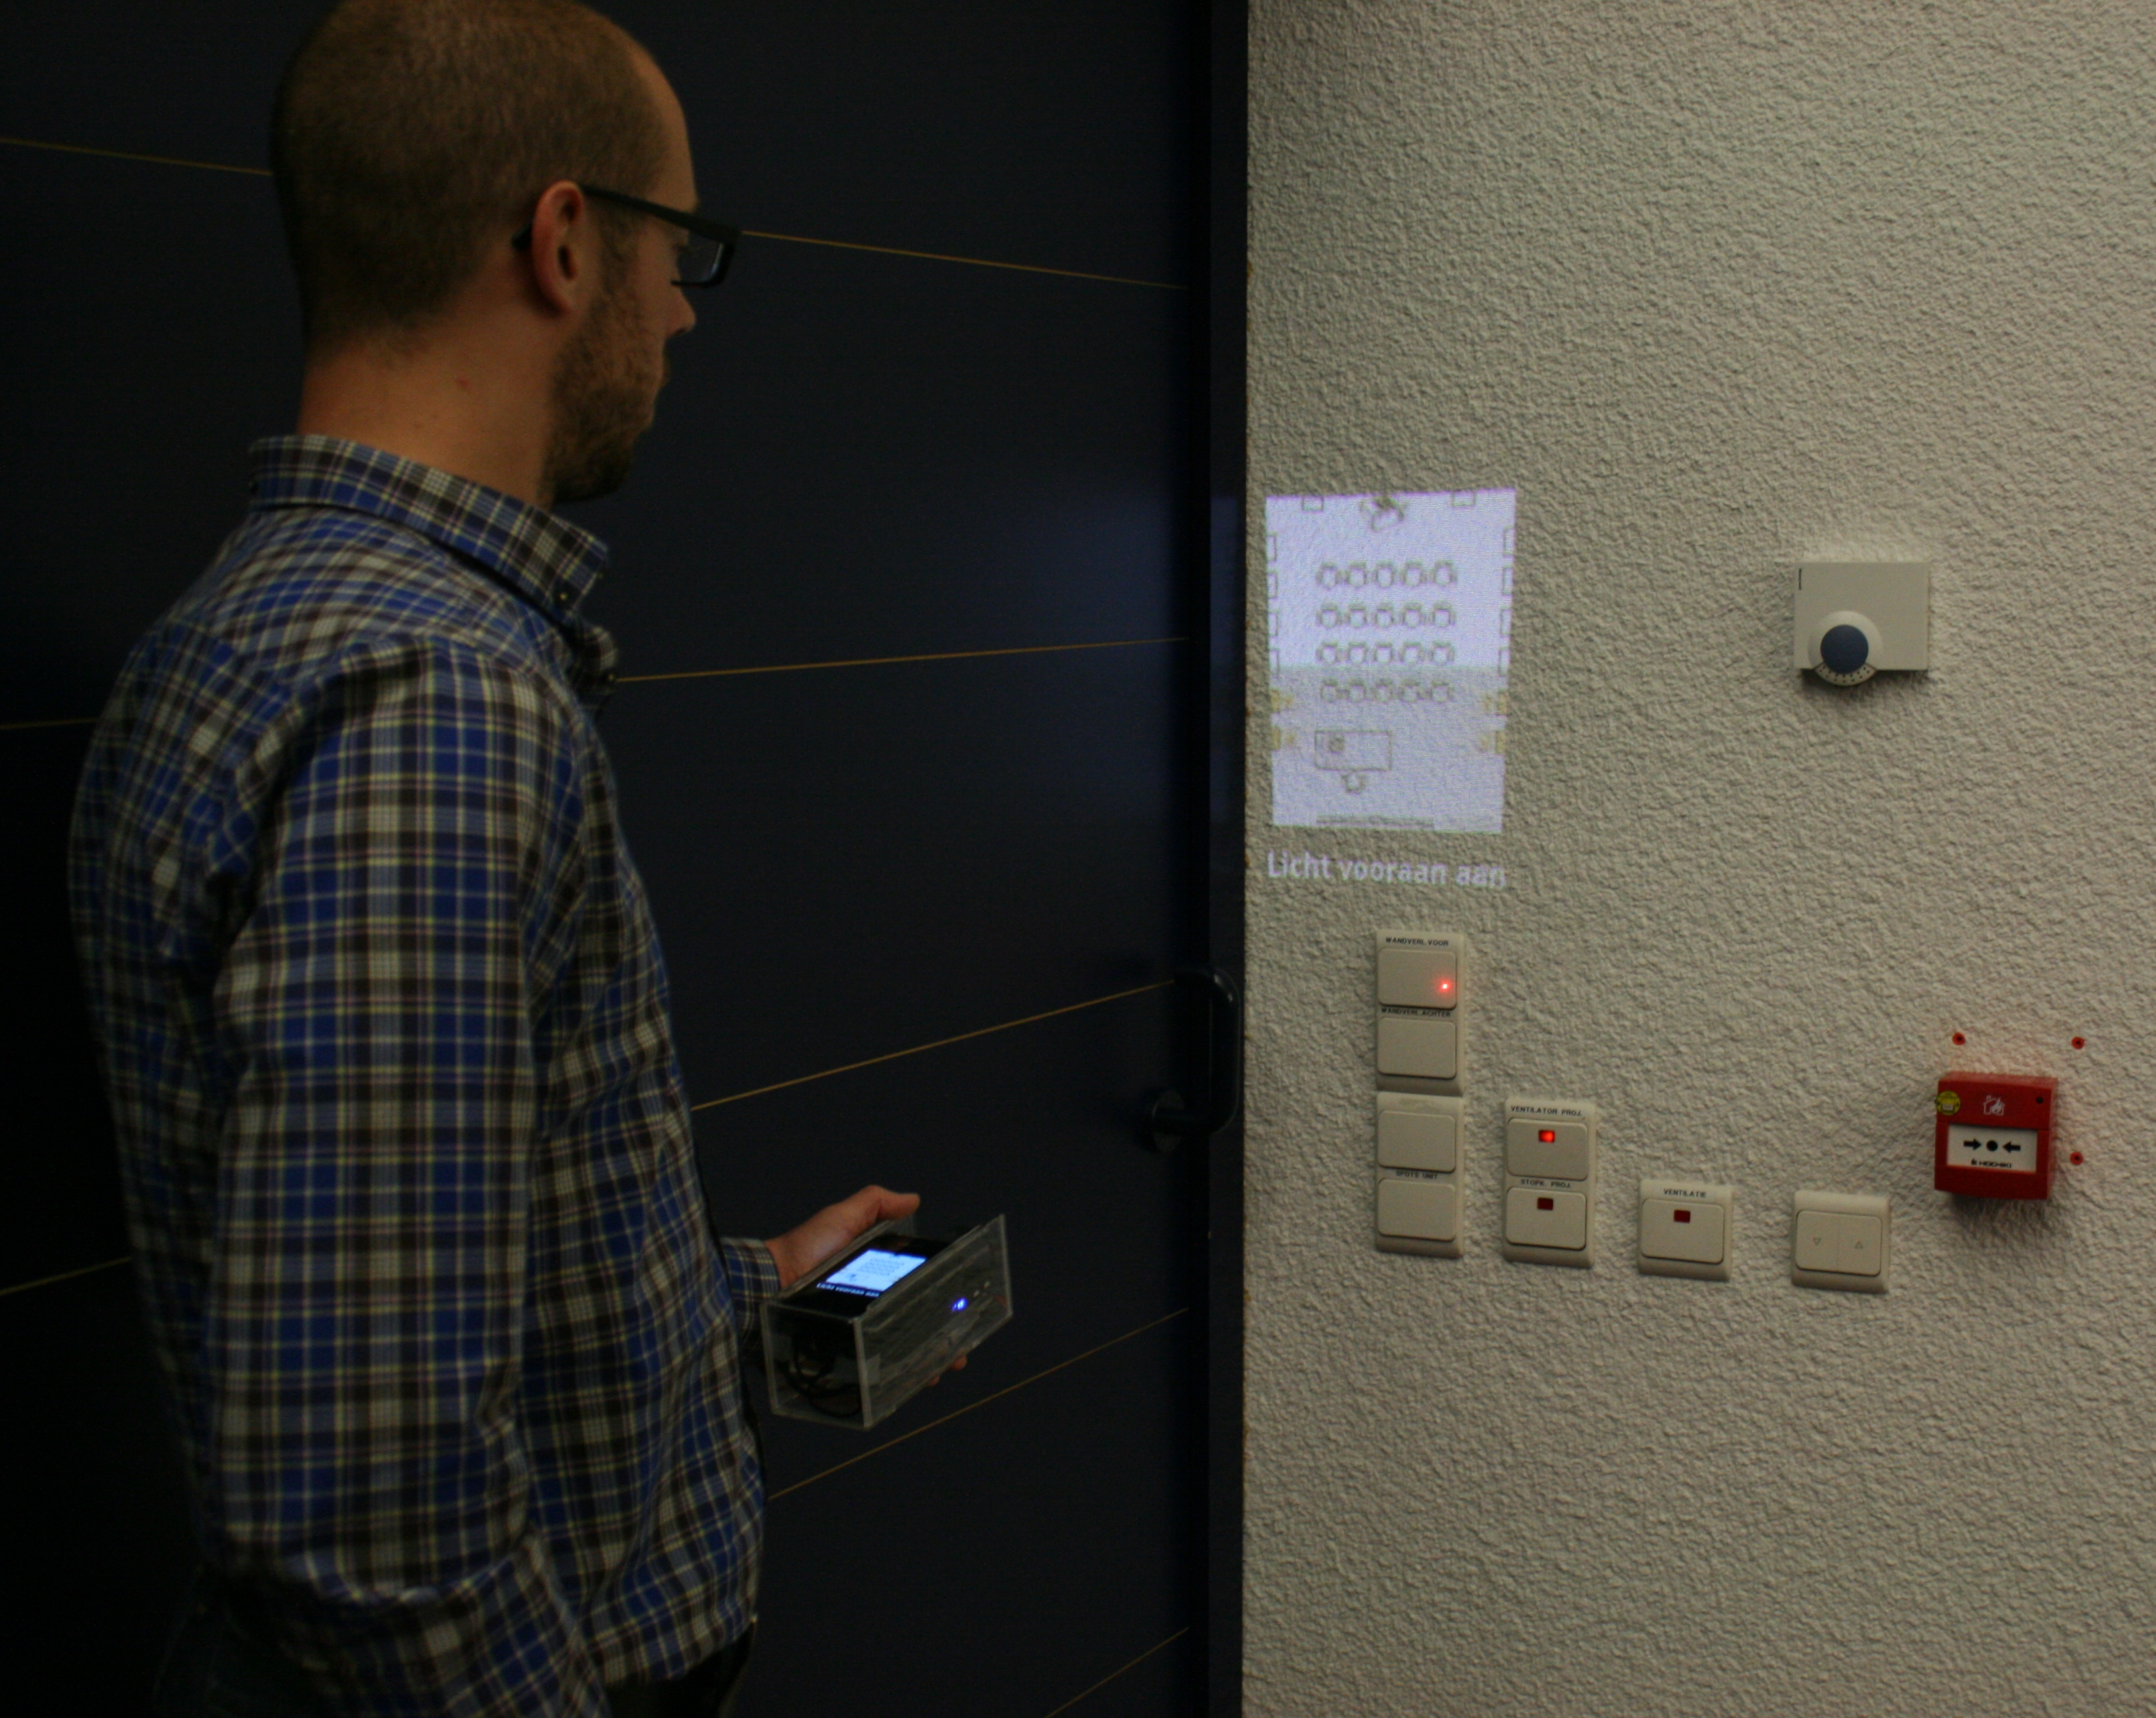
\includegraphics[width=0.6\linewidth]{img/park2014previewable/demo.png}
%	\caption{Product breakdown structure diagram.}
%	\label{fig:bps}
%\end{figure}
%
%\section{Scenarios} \label{section_scenarios}
%Many scenarios can be imagined where AR improves user experience by constituting feedforward. We divide these scenarios up into two categories, namely `setups in dumb environments' and `setups in smart environments', and for both of them, we discuss their advantages and give some examples.
%
%\subsection{Setups in Dumb Environments} \label{subsection_setups_in_dumb_environments}
%In these scenarios, the AR system cannot communicate with any other nearby systems. Often, this is because the nearby systems are simply not intelligent, but other reasons can also be thought of, like a lack of middleware required for communication. The AR system thus cannot change the environment and has to rely solely on its on-board sensors to gather information about its surroundings. To aid the system in this task, visual cues, e.g. QR codes, may be present.
%
%These setups are worth exploring because they are...
%\begin{itemize}
%    \item \textbf{low-cost}; the only material required is the AR system itself, plus potentially a set of visual cues, which come at any price, since they work just fine when printed in grayscale on plain paper.
%    \item \textbf{easy to set up}; no installation of peripherals is required, only the positioning of visual cues, if any.
%    \item \textbf{portable}; because setting up requires little to no work, moving to a different location is also easy. The setup can even exist simultaneously in different locations with little extra cost, since only the visual cues need to be duplicated, rather than having to buy and install multiple sets of peripherals.
%    \item \textbf{adaptable}; since setting up does not include careful installation of peripherals, changes are made more easily. What's more, if the AR system relies solely on visual cues for recognizing elements of interest, moving these cues suffices to relocate the elements, and adding more instances of an existing element is done by just creating more copies of its visual cue.
%    \item \textbf{noninvasive}; in some environments, like certain cultural heritage sites, drilling holes in the walls to hide peripherals and cables is unacceptable, and leaving them in plain sight spoils the view. Visual cues, on the other side, can be designed to blend in with the environment or, even better, can be comprised of objects already present.
%    \item \textbf{disposable}; in some contexts, people damaging or stealing peripherals can be a real concern. Especially in large outdoor or public areas, setting up expensive equipment may be deemed risky. Cheap, disposable visual cues can form a solution to this problem.
%\end{itemize}
%
%As a first example, let's consider a large museum, with several floors and many rooms. The museum currently provides audio guides, which are handheld devices that visitors carry with them for the duration of their stay. Every object of interest in the museum has a plaque with a unique number on it that visitors enter into their guides to hear a pre-recorded explanation about the object in question. This way, every visitor can finish the tour in any order they please, skip parts at will, hear explanations in their own language and replay them as often as they like. When this system works well, visitors have a great personalized experience.
%
%Let's assume there's no budget to install peripherals throughout the museum, because there are just way too many rooms. Even then, the museum is particularly well suited to be retrofitted for AR; procedures and infrastructure for handing out a personal device to every visitor are already present, and every object of interest already has a unique visual cue, mounted in a clearly visible location. Experiments must indicate if these existing number plaques can be recognized reliably by the AR systems, but even if they can't, another set of plaques can be installed when the old ones are due for replacement anyway, to save costs.
%
%In the museum, there are many ways in which AR can improve user experience, from highlighting relevant parts of objects during explanations, to small mini-games that can make the tour more engaging to children. However, we will not discuss these applications in more detail since our focus is specifically on feedforward.
%
%Imagine a visitor approaches an object of interest to take a closer look at it. The AR system detects this and displays a teacher icon in the user's peripheral vision to indicate that the associated explanation will shortly autoplay if the user does not interrupt. This is a perfect example of how AR can use feedforward to improve user experience, providing information about the near future without interrupting the user's current action.
%
%The visitor is now finished with the current room and wonders where to go to next. They look around and see three different exits, but can't remember where they've come from. In fact, they've just been wandering around the museum, pausing only at objects that caught their eye. This is where AR feedforward comes into play. Next to every door in the museum a unique painting is mounted, high enough as to always be visible and large enough to be recognizable from across the room. The AR system can now uniquely identify every exit in the building using these paintings, and augment the exits with personalized information. When the user looks to each of the exits, they receive variations on the following personalized information, displayed in some graphical or textual manner:
%\begin{itemize}
%    \item 3/12 visited
%    \item 2 recommended for you
%    \item this is where you come from
%\end{itemize}
%
%Since the AR system sees everything the user sees, it knows which objects the user has already visited, and assuming it has an internal model of the museum, it can deduce how many unvisited objects are left in each room. It can also make educated guesses about which unvisited objects would be particularly interesting to the user based on how much time they've spent observing related objects. Third, the AR system can track the user's path throughout the museum, even if they don't pause at any objects, by picking up visual cues along the way, since just a flash of a number plaque or a painting suffices to deduce the user's current location. An on-board GPS receiver can complement this data for even better reliability. Knowing the user's path, the AR system can show the user where they've come from to help them orient themselves.
%
%Displaying this kind of information about different rooms constitutes feedforward because it tells the user what will happen if they enter these rooms: whether they'll find new objects, whether they'll find objects that are likely to interest them, and whether they'll move forward or retrace their steps.
%
%The previous examples where chosen specifically because they are personalized, and thus different for each user. If instead we wanted to show users when special events would start in each room, or how crowded each room is (which we could determine if every AR system would transmit their location via a local network), one could argue that conventional displays work just as well, because the information shown is not user-dependent. However, if we wanted to show personalized information using a conventional display, it would have to cycle through the information of different users, possibly forcing some of them to wait their turn. What's more, the information would not be conveyed in a private manner, as others could also watch. In contrast, by using AR systems, an unlimited number of users can look at the same exit simultaneously and all see different data, without any of them having to worry accidentally sharing their information with others.
%
%% mention the value of these analytics to the museum
%
%[more examples]
%
%\subsection{Setups in Smart Environments} \label{subsection_setups_in_smart_environments}
%In these scenarios, the AR system is able to communicate with its environment; it can trigger changes in its surroundings and it can augment the input from its own sensors with data received from peripherals. Just like in the other category of scenarios, visual cues may be present here to aid the AR system in determining its location or identifying elements of interest, but they are certainly not the only means to do so.
%
%These setups are worth exploring because they are...
%\begin{itemize}
%    \item \textbf{powerful}; the ability of users to change the environment via virtual interfaces opens up a whole new range of possible applications (which we will illustrate in the examples).
%    \item \textbf{accurate}; using motion tracking systems, the user's position and orientation can often be determined with much greater accuracy than with the AR system's on-board sensors. This can reduce the number and severity of visual glitches, and it can make the AR system less dependent on visual feedback, which is particularly useful in low light conditions or when the view becomes obstructed.
%\end{itemize}
%
%[examples]

\clearpage
\bibliography{main}
\bibliographystyle{plainnat}

\end{document}
